\chapter{Important Concepts}
\label{chap:ic}

This appendix is a collection of important mathematical concepts that are frequently used in software engineering. 
The content of this appendix is based on the concepts in this book.

\begin{proposition}{Order of Operations}
To evaluate mathematical expressions, operations are performed in the following order:
\begin{enumerate}
    \item \textbf{Brackets (Parentheses):} First, perform all operations inside brackets or parentheses.
    \item \textbf{Exponents and Radicals:} Next, evaluate exponents (powers) and radicals (roots).
    \item \textbf{Multiplication and Division:} Then, perform multiplication and division from left to right.
    \item \textbf{Addition and Subtraction:} Finally, execute addition and subtraction from left to right.
\end{enumerate}
\end{proposition}

\begin{proposition}[Rules for Calculations with Fractions]
For $a,b,c,m \in \mathbb{R}$, with $a,b,c,m \neq 0$ where required, the following identities hold:
\begingroup
\setlength{\jot}{8pt} % increase space between align rows (default ~3pt)
\begin{align*}
(1) & \quad \frac{a}{b} \times m = \frac{am}{b} \\
(2) & \quad \frac{a}{b} \div m = \frac{a}{bm} \\
(3) & \quad m \div \frac{a}{b} = \frac{mb}{a} \\
(4) & \quad \frac{a}{b} \times \frac{c}{a} = \frac{c}{b} \\
(5) & \quad \frac{a}{b} \div \frac{c}{a} = \frac{a^2}{bc} \\
(6) & \quad \frac{a}{b} = \frac{ac}{bc} \\
(7) & \quad \frac{a}{b} + \frac{c}{a} = \frac{a^2 + bc}{ab}
\end{align*}
\endgroup
\end{proposition}

\begin{proposition}{Properties of Integer Exponents}
Let $n,m\in\mathbb{Z}$. Then the following hold (with $x,y\in\mathbb{R}$ and nonzero where stated):
\[
\begin{aligned}
&\text{(1)}\quad x^{n}\cdot x^{m}=x^{\,n+m},\\[2pt]
&\text{(2)}\quad \dfrac{x^{n}}{x^{m}}=x^{\,n-m}\quad \text{with } x\neq 0,\\[2pt]
&\text{(3)}\quad x^{n}\cdot y^{n}=(xy)^{n},\\[2pt]
&\text{(4)}\quad \dfrac{x^{n}}{y^{n}}=\left(\dfrac{x}{y}\right)^{n}\quad \text{with } y\neq 0,\\[2pt]
&\text{(5)}\quad \bigl(x^{n}\bigr)^{m}=x^{\,nm},\\[2pt]
&\text{(6)}\quad x^{1}=x.
\end{aligned}
\]
\end{proposition}

\begin{proposition}{More Properties of Integer Exponents}
Let $n,m\in\mathbb{Z}$. Then the following hold (with $x,y\in\mathbb{R}$ and nonzero where stated):
\[
\begin{aligned}
&\text{(7)}\quad x^{0}=1   &\qquad&   x \neq 0  \\
&\text{(8)}\quad \frac{1}{x^{m}}=x^{-m} &\qquad& x \neq 0 \\
\end{aligned}
\]
\end{proposition}

\begin{custombox}{Rules for rearranging formulae}
The following operations can be performed on both sides of the formula:
\begin{itemize}
    \item Add the same quantity to both sides
    \item Subtract the same quantity from both sides
    \item Multiply both sides by the same quantity - remember to multiply all terms
    \item Divide both sides by the same quantity - remember to divide all terms
    \item Apply a function to both sides, such as squaring or finding the reciprocal
\end{itemize}
\end{custombox}

\begin{definition} {Injective and Surjective Functions}
A function \( f: A \rightarrow B \) is called \textbf{one-to-one} (or \textbf{injective}) if different elements in \( A \) map to different elements in \( B \). 
A function \( f: A \rightarrow B \) is called \textbf{onto} (or \textbf{surjective}) if every element in \( B \) is the image of at least one element in \( A \).
\end{definition}

\begin{definition}{Inverse Functions}
Let $f$ be a one-to-one correspondence from the set $A$ to the set $B$. The inverse function of $f$ is the function that assigns to an element $b$ belonging to $B$ the unique element $a$ in $A$ such that $f(a)=b$. The inverse function of $f$ is denoted by $f^{-1}$. Hence, $f^{-1}(b)=a$ when $f(a)=b$.    
\end{definition}

\begin{figure}[htbp]
    \centering
    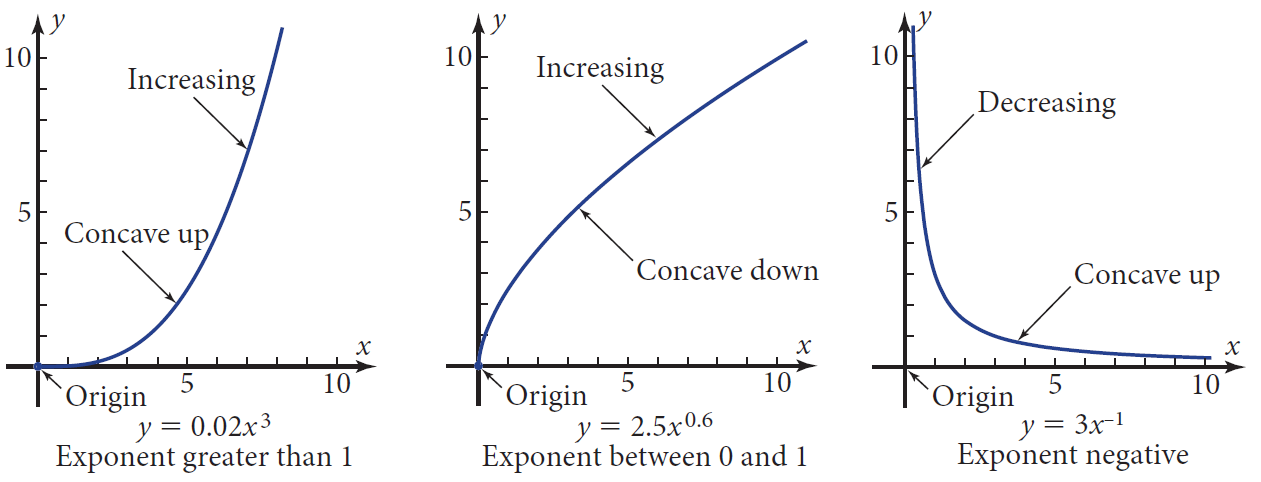
\includegraphics[width=1\textwidth]{figure/book3.png} % Adjust width here to scale the image
    \caption{Power functions}
\end{figure}

\begin{figure}[htbp]
    \centering
    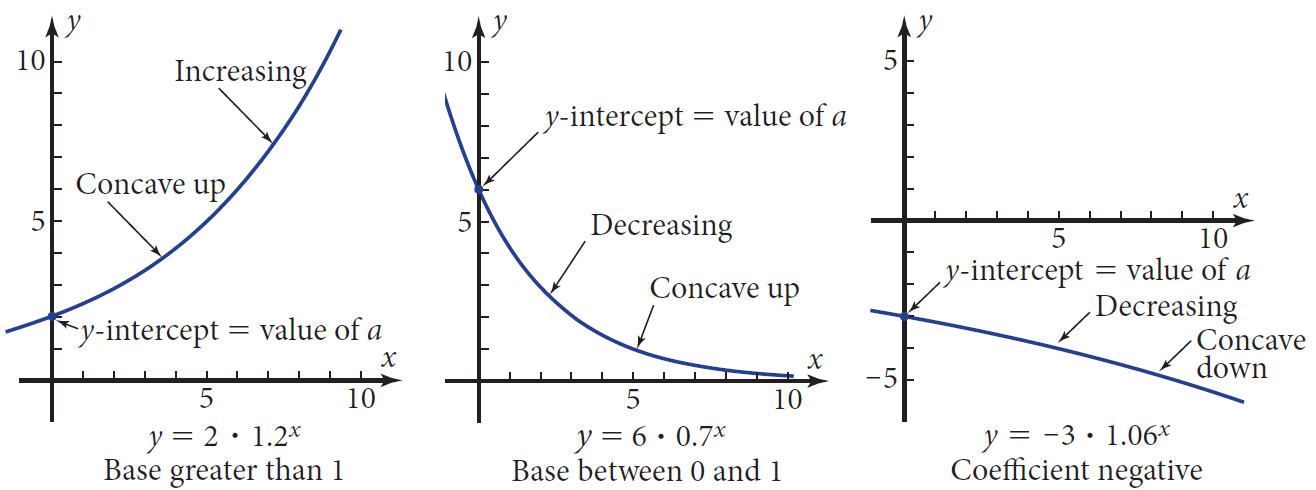
\includegraphics[width=1\textwidth]{figure/book4.png} % Adjust width here to scale the image
    \caption{Exponential functions}
\end{figure}

\begin{definition}{Base-10 Logarithms}

\[
\log x=y \iff 10^y=x
\]

\textit{Verbally}: $\log x$ is the exponent in the power of 10 that gives $x$   
\end{definition}

\begin{custombox}{Properties of base-10 logarithms}
\begin{itemize}
    \item Log of a Product:
    
    \[
    \log x y=\log x+\log y
    \]
    
    \textit{Verbally}: The $\log$ of a product equals the sum of the logs of the factors.
    \vspace{0.2cm}
    \item Log of a Quotient:
    
    \[
    \log \frac{x}{y}=\log x-\log y
    \]
    \vspace{0.1cm}
    \textit{Verbally}: The $\log$ of a quotient equals the log of the numerator minus the $\log$ of the denominator.
    \vspace{0.2cm}
    \item Log of a Power:
    \[
    \log x^y=y \log x
    \]
    \textit{Verbally}: The $\log$ of a power equals the exponent times the log of the base.
\end{itemize}

   
\end{custombox}

\begin{definition}{Common Logarithm and Natural Logarithm}
\hspace{1cm} \textit{Common}: The symbol $\log x$ means $\log _{10} x$.

\hspace{1cm}  \textit{Natural}: \hspace{0.2cm}The symbol $\ln x$ means $\log _e x$, where $e$ is a constant equal to $2.71828182845 \ldots$
\end{definition}

\begin{custombox}{The Change-of-Base Property of Logarithms}

\begin{equation*}
\log _a x=\frac{\log _b x}{\log _b a} \quad \text { or } \quad \log _a x=\frac{1}{\log _b a}\left(\log _b x\right)
\end{equation*}
    
\end{custombox}

\begin{custombox}{Properties of Logarithms}
\setlength{\leftskip}{1cm}  % Reset the text indent
\setlength{\rightskip}{1cm} % Reset the right indent
The Logarithm of a Power:
$$
\log _b x^y=y \log _b x
$$
The Logarithm of a Product:
$$
\log _b(x y)=\log _b x+\log _b y
$$
The Logarithm of a Quotient:
$$
\log _b \frac{x}{y}=\log _b x-\log _b y
$$
\setlength{\leftskip}{0cm}  % Reset the text indent
\setlength{\rightskip}{0cm} % Reset the right indent

\end{custombox}

% Additions for Chapter 02: Number Systems

\begin{table}[ht]
\centering
\renewcommand{\arraystretch}{1.4}
\begin{tabular}{|c|c|c|c|}
\hline
\textbf{Numeral system} & \textbf{Symbols} & \textbf{Base} & \textbf{Additional information} \\ \hline
\textbf{Decimal} & 0-9 & 10 & - \\ \hline
\textbf{Binary} & 0, 1 & 2 & - \\ \hline
\textbf{Hexadecimal} & 0-9, A-F & 16 & $\mathrm{A} \equiv 10, \mathrm{B} \equiv 11, \mathrm{C} \equiv 12,$ $\mathrm{D} \equiv 13, \mathrm{E} \equiv 14, \mathrm{F} \equiv 15$ \\ \hline
\textbf{Octal} & 0-7 & 8 & - \\ \hline
\end{tabular}
\caption{Summary of Common Numeral Systems}
\label{tab:number_systems}
\end{table}

\begin{table}[!ht]
\centering
\renewcommand{\arraystretch}{1.4}
\begin{tabular}{|c c c c c c c c|}
\hline 
\multirow{2}{*}{Decimal number} & & \multirow{2}{*}{In powers of 2} & \multicolumn{4}{c}{Power of 2} & \multirow{2}{*}{Binary number} \\
& & & 3 & 2 & 1 & 0 & \\ \hline
8 & $=$ & $2^3$ & 1 & 0 & 0 & 0 & 1000 \\
7 & $=$ & $2^2 + 2^1 + 2^0$ & 0 & 1 & 1 & 1 & 111 \\
6 & $=$ & $2^2 + 2^1$ & 0 & 1 & 1 & 0 & 110 \\
5 & $=$ & $2^2 + 2^0$ & 0 & 1 & 0 & 1 & 101 \\
4 & $=$ & $2^2$ & 0 & 1 & 0 & 0 & 100 \\
3 & $=$ & $2^1 + 2^0$ & 0 & 0 & 1 & 1 & 11 \\
2 & $=$ & $2^1$ & 0 & 0 & 1 & 0 & 10 \\
1 & $=$ & $2^0$ & 0 & 0 & 0 & 1 & 1 \\ \hline
\end{tabular}
\caption{Decimal Numbers in Binary Representation}
\end{table}

\begin{proposition}{Binary Addition Rules}
\[
0 + 0 = 0, \quad 0 + 1 = 1, \quad 1 + 0 = 1, \quad 1 + 1 = 10
\]
\end{proposition}

\begin{proposition}{Binary Multiplication Rules}
\[
\begin{aligned}
& 0 \times 0=0 \\
& 0 \times 1=0 \\
& 1 \times 0=0 \\
& 1 \times 1=1 \\
& 1 \times 10_2 = 10_2 \quad \left( \text{multiplying by base } 10_2 \text{ adds a 0 to the end} \right)
\end{aligned}
\]
\end{proposition}

\begin{proposition}{XOR Operation}
XOR produces a 1 if the two bits being compared are different and a 0 if they are the same:
\[
0 \oplus 0 = 0, \quad 0 \oplus 1 = 1, \quad 1 \oplus 0 = 1, \quad 1 \oplus 1 = 0
\]
\end{proposition}

\begin{figure}[htbp]
\centering
\begin{tikzpicture}[>=Stealth, node distance=4cm, thick, scale=1]

    % Draw larger circles for sets A and B
    \draw[thick] (0,0) circle [radius=1.5cm] node at (0, 2) {\Large $A$};
    \draw[thick] (6,0) circle [radius=1.5cm] node at (6, 2) {\Large $B$};

    % Place larger nodes for elements a and b=f(a)
    \node[fill, circle, inner sep=2pt, label=below:{$a$}] (a) at (0,0.3) {};
    \node[fill, circle, inner sep=2pt, label=below:{$b=f(a)$}] (b) at (6,0.3) {};

    % Draw the larger straight arrow representing f
    \draw[->, ultra thick, black] (a) -- (b) node[midway, above] {\Large $f$};

    % Draw the curved arrow representing f at the bottom, touching the circles
    \draw[->, ultra thick, black, bend right=30] ([shift={(270:1.5cm)}]0,0) 
    to node[midway, below] {\Large $f$} 
    ([shift={(270:1.5cm)}]6,0);

\end{tikzpicture}
\caption{A function \(f\) mapping an element \(a\) from set \(A\) to an element \(b=f(a)\) in set \(B\).}
\label{fig:function_mapping}
\end{figure}

\begin{figure}[htbp]
\centering
\begin{tikzpicture}[>=Stealth, thick, scale = 1.5]

% Draw circles representing sets A and B
\draw (0,0) circle (1.5cm);
\draw (6,0) circle (1.5cm);

% Labels for sets A and B
\node at (0,-1) {A};
\node at (6,-1) {B};


% Points in sets with adjusted labels
\node[fill=black, circle, inner sep=1.5pt, label={[xshift=-0.6cm]below:{$a = f^{-1}(b)$}}] (A1) at (0,0.7) {};
\node[fill=black, circle, inner sep=1.5pt, label={[xshift=0.5cm]below:{$b = f(a)$}}] (B1) at (6,0.7) {};


% Arrows for f and f^{-1}
\draw[->] (A1) to[bend left=30] node[midway, above] {$f(a)$} (B1);
\draw[->] (B1) to[bend left=30] node[midway, below] {$f^{-1}(b)$} (A1);

% Arrows for f and f^{-1} below the main circles
\draw[->] (0.6,-1.5) to[bend left=20] node[midway, above] {$f$} (5.4,-1.5);
\draw[->] (5.4,-1.8) to[bend left=20] node[midway, below] {$f^{-1}$} (0.6,-1.8);

\end{tikzpicture}
\caption{The function $f^{-1}$ is the inverse of function $f$.}
\label{fig:inv}
\end{figure}

\begin{figure}[htbp]
\centering
\begin{tikzpicture}[>=Stealth, thick]

% Draw circles representing sets A, B, and C
\draw (0,0) circle (1.5cm);  % Set A
\draw (5,0) circle (1.5cm);  % Set B
\draw (10,0) circle (1.5cm); % Set C

% Labels for sets A, B, and C
\node at (0,-1) {A};
\node at (5,-1) {B};
\node at (10,-1) {C};

% Points in sets with adjusted labels
\node[fill=black, circle, inner sep=1.5pt, label={[xshift=-0.1cm]below:{$a$}}] (A) at (0,0.7) {};

\node[fill=black, circle, inner sep=1.5pt, label=below:{$g(a)$}] (B) at (5,0.7) {};
\node[fill=black, circle, inner sep=1.5pt, label={[xshift=0.4cm]below:{$f(g(a))$}}] (C) at (10,0.7) {};

% Arrows for g and f
\draw[->] (A) to[bend left=15] node[midway, above] {$g(a)$} (B);
\draw[->] (B) to[bend left=15] node[midway, above] {$f(g(a))$} (C);
\draw[->] ([shift={(360:1.5cm)}]0,0) to node[midway, below] {$g$} (3.5,0);
\draw[->] ([shift={(360:0cm)}]6.5,0) to node[midway, below] {$f$} (8.5,0);

% Arrows for f ∘ g and (f ∘ g)(a)
\draw[->] (A) to[bend left=40] node[midway, above] {$(f \circ g)(a)$} (C);
% Draw the curved arrow representing f at the bottom, touching the circles
\draw[->, bend right=20] ([shift={(270:1.5cm)}]0,0) to node[midway, below] {$f(g(a))$} ([shift={(270:0.7cm)}]10,0);

\end{tikzpicture}
\caption{The composition of functions \(f\) and \(g\), denoted \(f \circ g\), is the function that results from applying \(g\) and then \(f\).}
\label{fig:composition}
\end{figure}

